The purpose of this work is to study the Fourier transform for its viability as a pitch detector. The FFT for transforming a waveform into the frequency domain has been introduced, and this chapter will focus on the properties of sound, introduce some musical terminology, and show how the FFT can be used to detect pitches from a time-domain signal.

\subsection{Basics of sound}
Sound physically is pressure propagation through a medium, a vibration that some things can produce, and some things can pick up. The word \textit{sound} can be used to describe both the propagation itself and the phenomenon we feel when our ears react to the propagation. Headphones, strings of a guitar, and vocal cords (together with the lungs) can produce sound. Microphones and ears can pick up sound \cite{RossingMooreWheeler}. The propagation will have a certain strength at some point in the medium it travels through, which can be measured. This allows us to model sound as a pressure change over time. At time $t$, the pressure at some point can be denoted as $f(t)$. This function over time can also be called a signal.

One simple way to generate sound is to connect a speaker to a device that generates an analog current in the shape of a wave. The current, using an electromagnet, moves a membrane at the same frequency as the generator, causing the pressure difference around the membrane. This membrane displaces air at some rate which ears pick up as sound. For example, if the generator produces a 440Hz signal, the speaker's membrane will displace air at the same 440Hz. This displacement is propagated over air and is sensed by ears as a pitch we call A4. Interestingly, the purity of the signal makes it sound harsh, and it is noise in the signal that gives warmth and beauty to the note. This is formally called timbre, and it allows us to distinguish an A4 on a piano from an A4 on a guitar even though both are A4 sounds.

%https://eprints.hud.ac.uk/id/eprint/17816/1/Final_Thesis_-_November_2012.pdf why is this here?

\subsection{Music fundamentals} 
Music terminology can be hard to define without circular definitions. There's also quite a bit of overlap with the same word meaning different things depending on context. A possible starting point would be defining the octave which is the difference between two sounds where one sound has twice the frequency of the other and is the largest interval in Western music. If a sound oscillates at 440Hz, the sounds corresponding to 220Hz or 880Hz are an octave away. The octave interval is commonly further divided into 12 smaller intervals that are equal in length on a logarithmic scale. These smaller intervals are called semitones are the smallest intervals in Western music. Notes can be defined as the specific pitches that bound the semitone intervals. Out of these notes, seven are chosen to form a primary set of notes. These are called naturals. 

While \textit{octave} is used to describe the interval, it is also used to refer to the range of notes lying between the two notes. A common way to label musical pitches is to use a letter to represent the note name and a number to indicate which octave group it belongs to. This system is called Scientific Pitch Notation (SPN) and is used in Western music notation. It starts on a C and ends in either a B or an H, depending on the convention used. Figure \ref{fig:noteScale} shows the octave bounds and how notes are ordered within the octave.

\begin{figure}[ht]
    \centering
    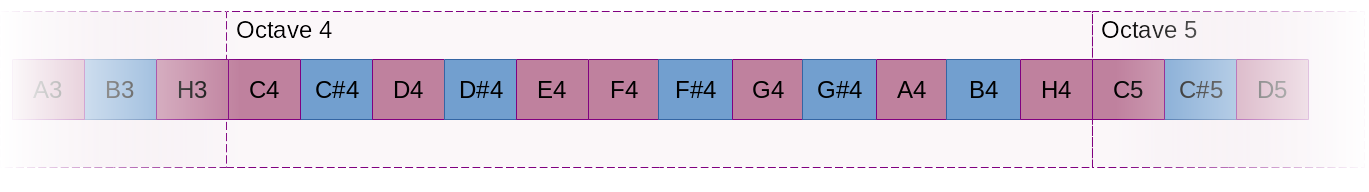
\includegraphics[width=\textwidth]{./images/noteScale.png}
    \caption{Notes of an octave. Natural notes are marked with purple. \label{fig:noteScale}}
\end{figure}

For example, the note which has twice (or half) the frequency of A4 forms an octave with A4. As the frequency is doubled, the other note is one octave higher than A4 so it is given the name A5. If the frequency is halved, it is named A3. 

In Western music, tuning typically starts from A4, which is defined in this system to have a frequency of 440Hz, and every other note is tuned relative to that. Tuning in this context essentially means finding the frequencies of the other notes so that everything sounds \textit{right} (to avoid getting into too much music theory). A3, an octave lower than A4, will be half of 440Hz i.e. 220Hz, and A5, an octave higher, will be 880Hz, which is double of 440Hz. The frequency for the other notes can be approximated with equal temperament tuning, meaning that all notes are equally spaced within octaves (logarithmically). This means that the frequency of any one note is exactly $2^{1/12}$ times the frequency of the previous one.  

\subsubsection{Flats and sharps}
Flats and sharps are augmented notes. Sharps are denoted with a $\#$ symbol and flats with a $\flat$ symbol. Both flats and sharps are one semitone offset to the augmented note meaning there is quite a bit of overlap. For instance, a D$\#$4 has the exact same pitch as a E$\flat$4. The key difference between D$\#$4 and E$\flat$4 is context. When \textit{playing in D-sharp}, there should be a D-sharp and not an E-flat even though they are the same pitch.

\subsubsection{Terminology for readers}
The natural notes will be defined according to German/European music theory as \[C, D, E, F, G, A, H\] and B being $H\flat$. In this work, the term \textit{note} will be used to describe the 12 distinct sounds within the octave because for the pitch detector, discerning the natural notes and the sharps and flats is not of importance. The term \textit{pitch} will be used to describe the measurement/perception of how low or high a sound is.

\subsubsection{MIDI numbers}
For humans, it is easy to use the SPN labels for notes. C4, for example, is a simple pair of a letter and a number and gives users sufficient information to know what it refers to. Computers, in contrast, are different and instead have it much more difficult to analyze the string "C4", even compared to pure frequencies. However, the frequency value is often unnecessary because we usually only care about a discrete set of frequencies corresponding to notes, not all possible real-valued frequencies. Musical Instrument Digital Interface (MIDI) is a technical standard for protocols, connectors, and interfaces relating to music and, among other things, assigns integers to notes. These integers have a direct mapping to both frequencies and to notes. For example, $A4 \sim 440\mathrm{Hz} \sim 69$.


% \subsubsection{Pitch perception}
% Even though we can clearly define any one pitch to be some frequency, human ears are more complex. 
% What do I want to establish in this chapter????
% What is pitch perception at a high level
% 
\subsection{Fundamental frequency estimation}
Even though we can define a pitch to be a precise frequency, pitch is more of a sensation perceived by ears, and we can distinguish pitch from sound waves that are not simple oscillations. What we perceive as the note A4 can contain a large amount of noise, or timbre. As it can be difficult to strictly define pitch, pitch detection may also be difficult to define. Pitch is, however, strongly tied to the fundamental frequency, which is the lowest perceived harmonic of a signal. Even though the timbre of a piano and a guitar are vastly different (which allows us to hear a difference between the two) if they play the same note, the fundamental frequency will be the same. 

From a computational perspective, a possible definition for pitch detection is the identification of the fundamental frequency. An additional computational aspect is to convert the frequency to SPN for user convenience. 

The fundamental frequency is typically the lowest frequency of a signal but, in some cases, we can hear a fundamental frequency that is not part of the signal, a phenomenon appropriately called the missing fundamental. \cite{Gotsopoulos}. An example of this would be smaller speakers, like those found in the handset of a phone, that could not produce sound below 300Hz. A male voice would still sound low, even though its fundamental frequency of around 150Hz was completely missing \cite{Mather2009}.

\subsubsection{The missing fundamental}
The missing fundamental is in a sense an auditory illusion. It is a result of the constructive interference of harmonics that causes peaks with a period that is the greatest common divisor of the angular frequencies of the harmonics. This is shown in Figure \ref{fig:missingfund} where the sum of several waves produces a wave with a prominent 110Hz oscillation. Even though the lowest frequency component is 220Hz, the prominent 110Hz oscillation is what we feel and hear.

\begin{figure}[ht]
    \centering
    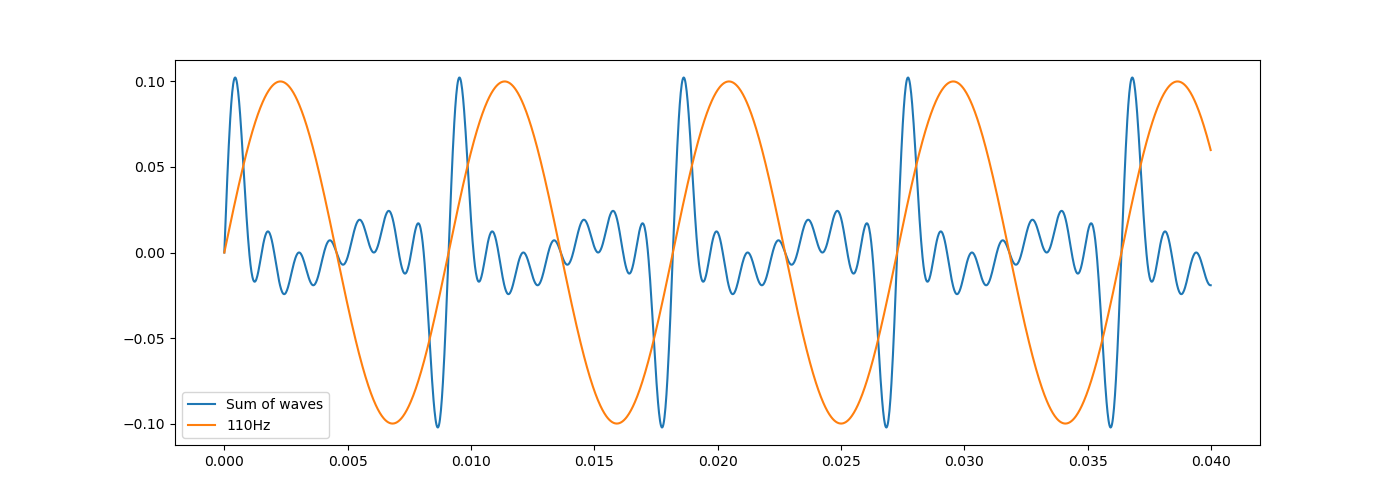
\includegraphics[width=\textwidth]{./images/missingfund.png}
    \caption{Constructive interference of harmonics creates the missing fundamental. Even though the blue signal only contains sinusoids with frequencies greater or equal to 220Hz, the most prominent part of the final signal has a period of 110Hz. \label{fig:missingfund}}
\end{figure}

Pipe organs use this to their advantage. Creating extremely low sounds requires enormous pipes. Taking advantage of the missing fundamental allows relatively smaller organs to produce low sounds \cite{Veritasium2024}.
% 0:56; https://www.youtube.com/watch?v=Sn07AMCfaAI&t=1169s

\subsection{Pitch detection methods}
Pitch detection methods typically fall into one of three categories: time-domain, frequency-domain, or statistical/machine learning methods. Some common time-domain methods include zero-crossing rate and autocorrelation. Zero-crossing rate is a method in which frequencies are extracted by keeping track of the rate at which the signal crosses the x-axis. Another is autocorrelation, in which the signal is compared to itself with a different phase. 

This thesis will focus on a frequency-domain approach, where a Fourier transform is used to create a representation of the sound that is easier to analyze and process.

\subsection{Transforming to frequency-domain}
The first step in detecting pitch using the frequency domain is to transform the original signal into the frequency domain, and there are multiple ways to achieve that. The DFT and FFT were already introduced in the introductory Fourier analysis chapter, and as already established, some version of FFT should be used as the transformer since the DFT has terrible performance. 

Disregarding the question of how to process binary audio files—even if the data were decoded—how should the data be processed? If the whole audio signal is given to the FFT, the spectrum will be a complete mess because real music or song contains more than a single note or chord.

\subsubsection{Short-time Fourier Transform}
The short-time Fourier transform (STFT), sometimes also called the windowed Fourier transform, is a method of analyzing a signal by looking at parts of the signal. The STFT is typically defined very similarly to the FT/DFT, but with a windowing function applied. The continuous STFT is usually defined as the following

$$S(x(t), \tau, \omega ) = \int_{-\infty}^{\infty} x(t)W(t-\tau)e^{-i\omega t}dt$$

\noindent where $x(t)$ is the input signal, and $\tau$ is the center of the window function $W$. The window function may be freely chosen, for example, a Gaussian window or a Hamming window. Conceptually, this is computing the transform for a signal $S_2$ that is some signal $S$ with a windowing function applied so that outside the window, the signal has 0 value. The window is then moved and the \textit{next} value is computed. The discrete STDFT conversely computes the DFT for just some chunk of a discrete signal. Like the STFT, it then moves the window over some number of steps (called the hop length in discrete context) and repeats. If the hop length is shorter than the window size, the windows will overlap.

This sliding window introduces a new dimension to the output data—a time axis. This data constitutes a spectrogram and the typical way to visualize this data is with a heat map by compressing the 2D frequency domain to a column where intensity represents the magnitude value for a frequency. Figure \ref{fig:stft} shows how the spectrogram is created.

\begin{figure}[ht]
    \centering
    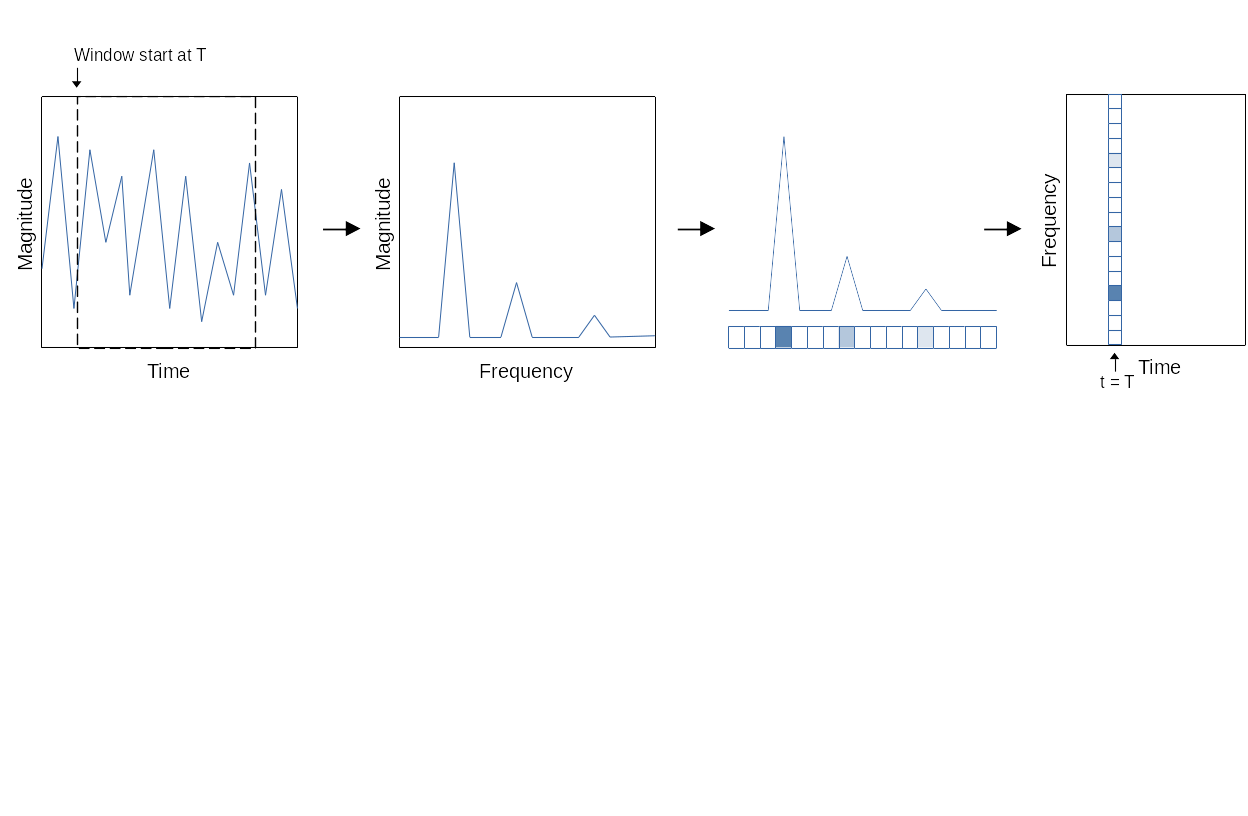
\includegraphics[width=\textwidth]{./images/stft.png}
    \caption{Diagram of how the STFT performs the DFT for one window which results in one column in the spectrogram. For ease of visualization, the frequency domain is typically visualized using color intensity for the magnitude. \label{fig:stft}}
\end{figure}

It is worth pointing out that the STFT is not a special kind of Fourier transform but rather a method of applying the DFT/FFT (or continuous FT). This means it exhibits the same behavior, but also that it has the same problems, which will be introduced shortly. 

For real-time processing, it is both essential and somewhat redundant to talk about the STFT because the entire signal is never available so there is no need for windowing. The data will be available as a stream (or chunks) and an FFT can be performed once a buffer is filled, after which the buffer is cleared. The buffer serves as the window, so as long as the transform is computed sufficiently often—which is necessary for real-time applications—the method, in a sense, implements a discrete STFT. The overlap, which is determined by the hop length, does not seem to be of much importance for the purpose of estimating the fundamental frequency and makes little sense when the data becomes available with time. The overlap is important when considering note lengths and separation of repeated semitones \cite{Evans2012}, but does not seem to be a concern for just pitch detection. Consequently, the pitch detector will have a hop length the size of the window—or in other words, no window overlap.

\subsection{Picking peaks from the spectrum}
The Fourier transform is used to obtain the spectrum data, which can be used to plot which frequencies are part of the original signal. These frequencies that are part of the signal are called partials. Intuitively, for a lot of signals, anyone can look at the frequency-magnitude plot, choose peak, and claim that it is the fundamental frequency—and they would probably be right. Perhaps they are looking at the spacing of the largest peaks (if there are multiple) and, out of the peaks that fit the spacing, choosing the one that has the lowest frequency. This is a very straightforward approach and correct for some signals. 

% HPS
\subsubsection{Harmonic Product Spectrum}
Harmonic Product Spectrum (HPS) is an algorithm that works similarly to the intuitive approach. It is defined as follows:

$$Y = \prod_{r=2}^R X_r$$

\noindent where $X_r$ denotes the signal $X$ downsampled by $r$. Simply put, the HPS iteratively multiplies downsampled version of a signal. Downsampling in the frequency domain effectively compresses the frequency axis by the downsampling rate which means that previously integer multiples of some value $kN$ end up in the same bins as $N$. When all the downsampled frequency-domain signals are multiplied together, correlated frequencies, or harmonics, form a very sharp peak \cite{McLeod2008}. This peak can be identified with a max function.

\begin{figure}[ht] \centering 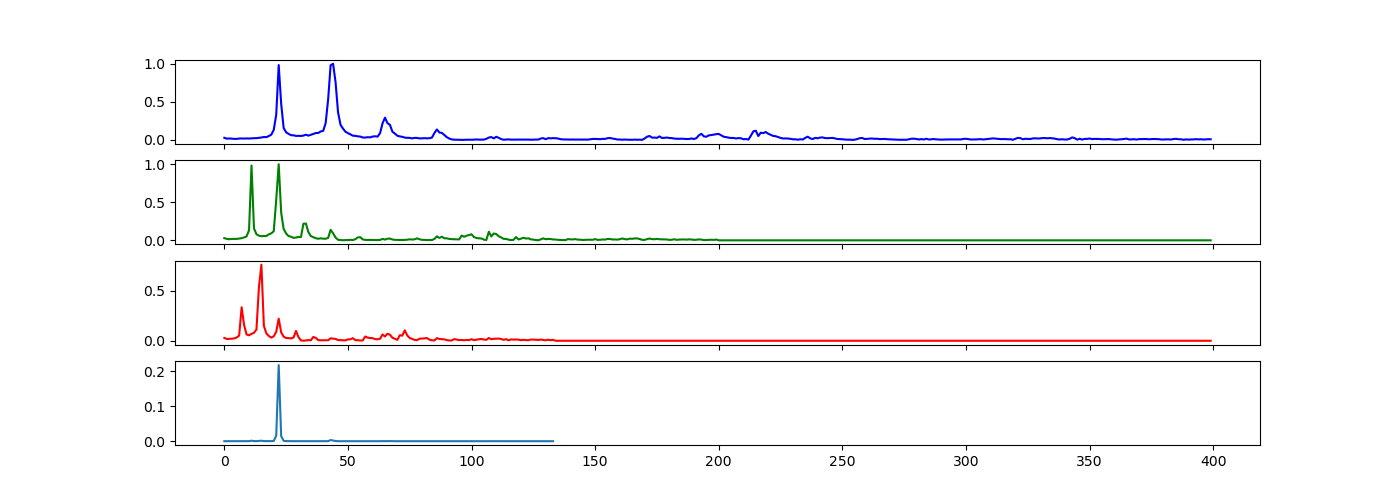
\includegraphics[width=\textwidth]{./images/hps.png} \caption{Plot of signal, downsampled versions of it, and the final HPS. The topmost signal is the original, the two middle time series are downsampled versions of the signal. The bottom-most signal is the frequency-wise product of the downsampled versions, i.e. the HPS. Harmonics align and form a peak. \label{fig:hps}}
\end{figure}

HPS is a promising algorithm because it is simple and easy to compute, making it suitable for real-time analysis. As the HPS essentially looks at the ratio of the harmonics, it can find a missing fundamental. Even if the fundamental is part of the spectrum, it may not always be the strongest, in which case the HPS helps by enhancing it for easier discernment from noise.

The biggest problem with the HPS is that it does not perform well in the case of lacking harmonics \cite{McLeod2008}. This is likely not  a problem because human voices should be rich in harmonic content. In the more extreme case, where noise is dominating, the system would still compute the HPS and one largest peak would form somewhere, resulting in garbage data. A possible way to mitigate this is to check the spectral flatness (sometimes called tonality) of the signal and ignore the result if the flatness is too high. HPS is also prone to getting octaves wrong \cite{Smyth2019}.
% CFAR
% https://www.youtube.com/watch?v=BEg29UuZk6c
\subsubsection{Constant False Alarm Rate}
Constant False Alarm Rate (CFAR) is an algorithm that gives a dynamic threshold. It works by looking at some amount of reference cells that are beyond some gap around the target cell. For example, for cells 5, 6, 7, 8, 9, 10, 11, 12 and 13, the threshold given a gap size of 2 and reference cell count of 2 and the target is 9, the reference cells are 5, 6, 12 and 13, whereas 7, 8, 10 and 11 are gap cells. The reference cells are then averaged (but other statistical methods can be used) and a bias may be applied. If the value of cell 9 is above the computed threshold, it is considered a target, and noise if the value is below. CFAR is typically used in conjunction with radar technology but could just as well be used to discern the partials in a spectrum \cite{Bruner2024}. 

\begin{figure}[ht]
    \centering
    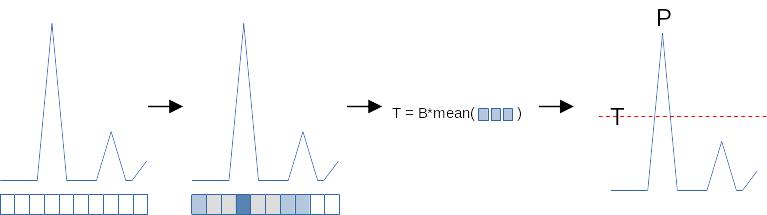
\includegraphics[width=\textwidth]{./images/cfar.png}
    \caption{Diagram of the CFAR algorithm with 2 gap cells and 2 reference cells. The gap cells around the target point P are excluded but the reference cells in light blue are used for calculations. The reference cells are averaged which gives the threshold T for point P. As P is greater than T, P is regarded as a target.\label{fig:cfar}}
\end{figure}

To effectively use CFAR, the parameters must be carefully chosen. If the bias is too low, invalid targets may be considered targets, and vice versa if the bias is too high. The gap and reference cells can be fairly flexible but not too large, as smaller harmonics may be considered noise compared to greater harmonics. The lowest pitch we want to estimate is around 50Hz and if we assume monophonic singing, the spectrum should only contain integer multiples of the fundamental frequency, which means that no peaks should ever be closer than 50Hz. With 4Hz bins, it is possible to use up to 12 gap and reference cells for the CFAR computations without ever having another frequency component be part of the reference cells.  

As CFAR only finds the peaks, one problem with using it alone as a fundamental frequency estimator is that additional post-processing is necessary. Since HPS already works well for extracting the fundamental frequency, it is chosen as the primary algorithm for the fundamental frequency estimator. CFAR could, however, be used to give a rough number for peaks, which may be used to dynamically adjust the number of iterations the HPS uses. If CFAR finds very few peaks or even just one, the result could be used to completely change the peak picker as HPS has issues with signals without harmonics.

% Problems with FFT, might move this to real-time
\subsection{Problems with the FFT}
One problem with the FFT that \cite{Gotsopoulos} addresses is the size of the frequency bins. This is also noted for the STFT, limiting how short the STFT can be for achieving sufficient frequency resolution \cite{Evans2012}. The FFT doesn't find precise frequencies, it finds bins of frequencies with the size $S/N$ where $S$ is the sampling rate and $N$ is the FFT buffer size. As frequency grows exponentially (doubles every octave), higher notes are spaced further apart. This means that for lower notes, the frequency bins need to be significantly smaller as shown in Figure \ref{fig:fftBinSizeChart}. Base singers may need to go very low, around E2 (87Hz), and in order to avoid notes in this range to fall into the same bin, the window size needs to be very small.  

\begin{figure}[ht]
    \centering
    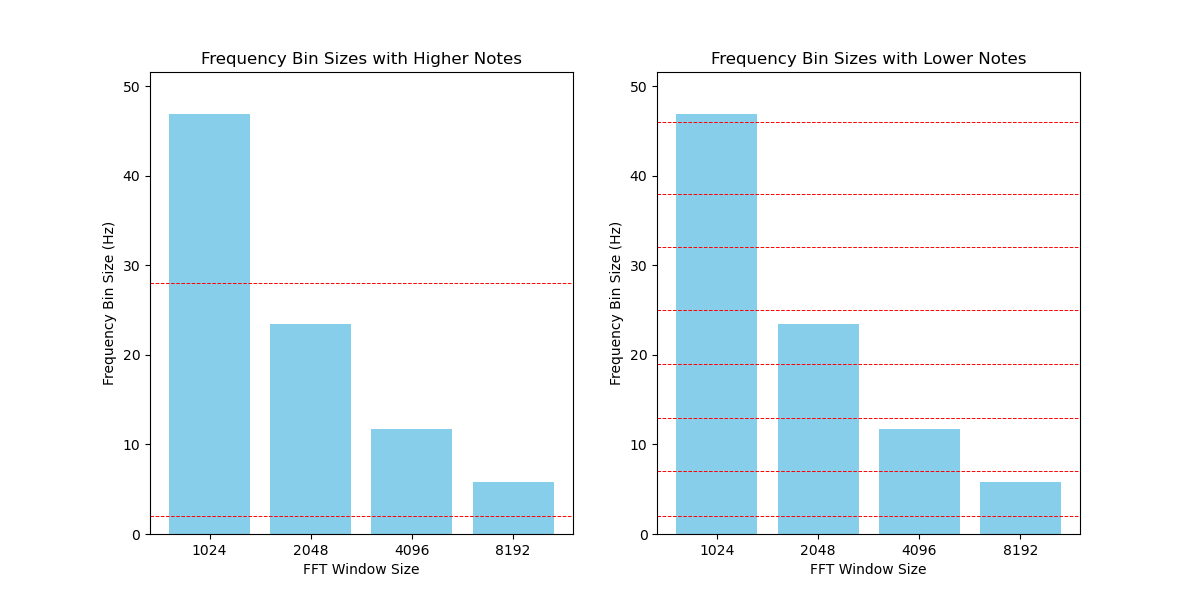
\includegraphics[width=\textwidth]{./images/fft_bin_size_chart.png}
    \caption{As the FFT window shrinks, different notes may fall into the same bin. Bars represent the bin sizes for various window sizes at 48kHz sampling rate and dashed lines show semitone intervals (the exact note values are irrelevant). For notes in the 4th octave, the window size can be smaller, but in the 2nd octave, even 8192 samples is not enough to discern all pairs of semitones because the bins are larger than those semitone differences.\label{fig:fftBinSizeChart}}
\end{figure}

Base singers typically go as low as E2 and the difference between E2 and F2 is barely 5Hz which is smaller than the frequency bin of 8192 samples at 48kHz. They do not necessarily fall into the same bin, but it would be safer to compute the FFT with a 16384 window size. This halves the frequency bin size and definitely accommodates differences even an octave lower. This introduces a significant amount of increased computation and is quite unnecessary as bass singers do not realistically go much lower than E2. If the FFT implementation allows (many implementations require a power of 2), the window size should lie somewhere between 8192 and 16384 to lessen computations. For a 4Hz bin, $48000/x = 4 \iff x = 48000/4 = 12000$, 12000 samples would be enough to discern the lowest notes. 

This introduces another problem, which has implications for real-time pitch detection, which is that collecting 12000 samples at 48kHz takes 0.25 seconds, which arguably is not real-time anymore. As the bin size is $B = S/W$ means that $W = S/B$ and the latency (time taken to fill the FFT window) $L = W/S = \frac{S/B}{S} = 1/B$, the bin size and latency are inversely proportional, both can not be minimized. For a bin size of 4, it will necessarily take 0.25s to collect the FFT samples. This follows that naively transforming audio makes real-time pitch detection for bass singers impossible because the detection latency will inherently always be too long with sufficiently fine frequency resolution.

% Note timings
\subsection{Note lengths and timings}
Note lengths are defined as fractions in relation to the beat. The beat is the recurring pulse of the music which relates to the tempo and the time signature. In common time (which is noted with 4/4), the beat is implied to have the same length as a quarter note. A whole note, thus, is sustained over 4 beats and similarly two eighth notes can be played in a single beat. Music is in other words always written using relative lengths and the overall speed is defined by the composer, often using natural language. The musician should respect the relative note lengths, but they may or may not respect the pace set by the composer.  

How a piece of music is performed often deviates considerably from how it was written. There are several reasons for this. For one, sheet music is not an algorithm but closer to natural language. Much is up for interpretation, most notably as far as pace and dynamics are concerned. When a musician encounters the tempo marking, for example, \textit{andante}, they just have to know and/or feel what it means because no consensus seems to exist about the precise tempo of \textit{andante}. Most sources give a range, but even the ranges are different between sources. Another term, \textit{accelerando} simply means to accelerate. By how much or how quickly is not specified. Musicians may ignore them completely and even make them up, to introduce their own touch to the performance. In the simpler case, some sections may just be dragged as the musician or conductor wants. Figure \ref{fig:performance-sheet} visualizes two time series using color intensity instead of magnitude. This is for demonstration purposes only, and what they are or how they were created is not of importance for the moment. The upper time series is the definition of the piece as the sheet music states. The time series below is one performance of the piece. The figure reveals how the pace in the rendition deviates from the sheet. It should be easy to see a strong similarity between the two. They are not quite identical, but their structure is identical, and they have similar substructures. 

\begin{figure}[ht]
    \centering
    
\includegraphics[width=\textwidth]{./images/performance-sheet.png}
    \caption{The time series of a piece as the sheet music suggests (above) and of a performance of said piece (below)\label{fig:performance-sheet}}
\end{figure}

\subsubsection{Time series similarity}
The similarity of two time series can be measured with Dynamic Time Warping. Understanding timing and DTW is important because it helps in understanding the computational problems in  creating a program that can compare sang notes to expected notes. As DTW works with a longer signal (as opposed to a single sample), it is not suitable for real-time detection. DTW is thus used for developing and testing the detector using recordings for consistency and convenience and is only a tool for the analysis of the notes detected by the pitch detector. 

% Narrowing the problem
\subsection{Real-time monophonic pitch detection}
The focus of this work is on real-time pitch detection, specifically for the purpose of rating and aiding a user in practicing their singing. To clarify, real-time means that the input of the system is a stream and the system processes small chunks as they come up and forget anything that it has already processed just like a human would listen to a short window in time, decide the pitch for that window and move on, not caring about the previous windows and not knowing anything of upcoming windows. The acceptable latency of \textit{real-time} is contextual. For rendering, it should be around 33 milliseconds to achieve 30 frames per second, whereas for real-time tracking in logistics, it is probably enough to update every minute or even hour. 

What real-time means in this particular context can be debated and studied further, but the goal is just that it is fast enough so that the user can react to their mistakes. This is akin to a teacher telling a student that they are off to give the student instant feedback, as opposed to saying something like “There was a mistake in the 3rd note in the 11th bar” which may be little to no help for a beginner. According to humanbenchmark.com, the mean reaction time is 284ms based on their collected 81M benchmarks \cite{HumanBenchmark2025}. The Human Benchmark benchmark is based on visual stimuli, but it is noted that the reaction to auditory stimuli is slightly faster \cite{SheltonKumar2010}. The goal for this work is significantly below the mean visual reaction time at around 100ms. In any case, even if humans can react to auditory stimuli faster than this, as the purpose is to give live feedback to the user on their own singing rather than having the user react to someone else's singing, the user is limited by their reaction speed to the feedback (which is visual stimuli).

% Zero padding
\subsubsection{Zero-padding}
One challenge with real-time pitch detection that emerged from the problem with the size of frequency bins was that for detecting lower bass notes, the window size needed to be around 12000. However, collecting 12000 samples at 48kHz takes 0.25s, which arguably is not real-time anymore. It takes 0.33s if for any reason the window size needs to be 16384. If the window size is made smaller, the resulting FFT may not have sufficient frequency resolution for the separation of lower frequencies. 

A popular approach to increasing frequency resolutions is to pad the end of the signal with zeros. Zero-padding makes the signal longer and while it necessarily introduces frequency components (more bins with a longer input signal), the peaks remain largely intact. A larger FFT window, while increasing computational complexity, allows for better frequency resolution. At 48kHz, 16000 samples are enough to achieve a 3Hz frequency bin. If out of these 16000, 10000 are zeros and 6000 legitimate data points, the FFT window can be filled in a mere 125ms which is a more acceptable latency for real-time detection. Figure \ref{fig:zeropadSpectrum} shows how zero-padding affects the spectrum.

\begin{figure}[ht]
    \centering
    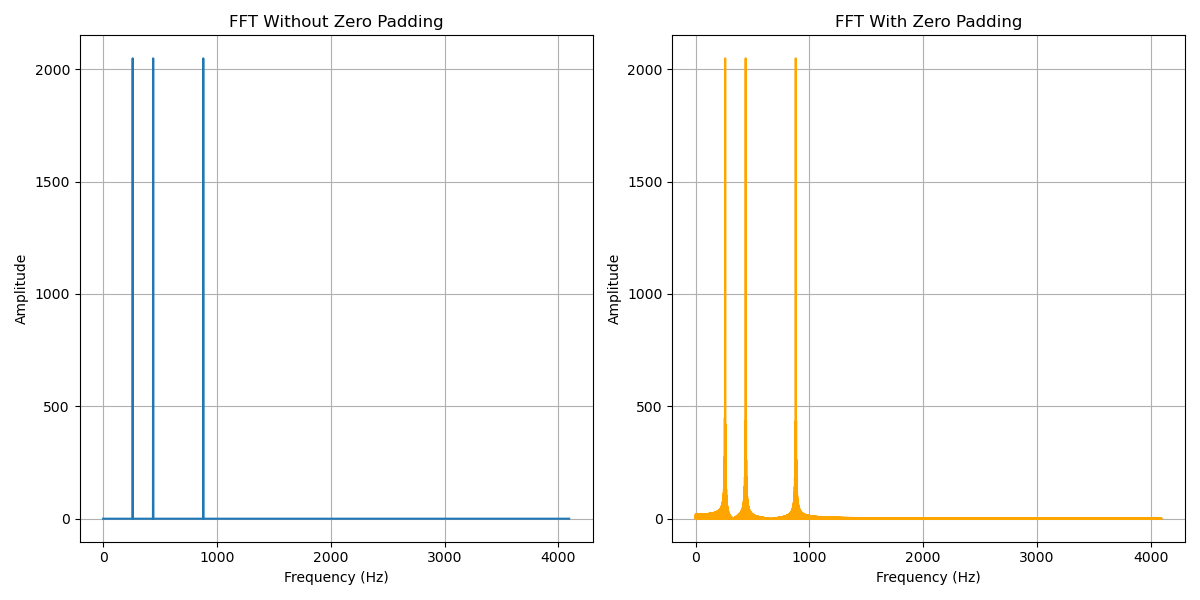
\includegraphics[width=\textwidth]{./images/zero_pad_spectrum.png}
    \caption{Spectrum contents of a signal consisting of 260, 440 and 880 frequency components. While the zero-padding introduces a small amount of frequency data around the peaks, the peaks themselves are not affected. \label{fig:zeropadSpectrum}}
\end{figure}

\subsubsection{Reducing sampling rate and window size}
As the bin size is the ratio of the sampling rate to the number of samples, $B = S/N$, reducing both $N$ and $S$ keeps the bin size small. If only the window size is reduced, the bins grow in size, and frequency resolution is lost. With zero-padding fixing the latency issue, why not reduce the sample rate as well to ease the computational load? Ignoring system limitations of the sampling rate — like Firefox not even supporting changing the sample rate for MediaTrack objects — another issue is aliasing. Aliasing, in short, is the misrepresentation of higher frequencies as lower frequencies. 

The Nyquist-Shannon sampling theorem states that there is no loss of information when sampling at $2B$ hertz if the signal contains frequency components that are less than $B$ hertz. It, thus, implies that if the sampling rate is lowered, higher frequencies may be misrepresented. For example, if a signal is sampled at 44.1kHz, the biggest frequency component that can be represented without ambiguity is 22050Hz, which is also called the Nyquist frequency for the given sample rate. If the signal contained a 30kHz component, which would exceed the Nyquist frequency, it would be perceived as a 14.1kHz component. This can be computed using $|s-f|$ where $s$ is the sample rate and $f$ is the frequency component. Conceptually, one could imagine drawing the frequency range on a piece of paper and literally folding it along the Nyquist frequency. After the fold, the 30kHz and 14.1kHz components would end up in the same position.

As the pitch detector in this work has no reason to play back the sound, the waveform can be processed in almost any way as long as no crucial information is lost or skewed. Compared to the lowest male voices, there seems to be less consensus on the highest female voice, but a pitch higher than G6 at around 1567Hz seems to be uncommon. A more typical highest note is C6 at around 1046Hz. To be on the safe side, the ability to detect 1567Hz components can still be considered a valid requirement. If the pitch detector needs to detect a 1567Hz frequency, the sampling rate needs to be no smaller than 3134Hz. However, the human voice is rich in harmonics, if these are aliased, they will be presented as lower notes which in the best case would get the octave wrong and in the worst case get completely wrong notes.

The sampling theorem clearly states what we can and can not do with the signal, but it all depends on the harmonics of voices. Clearly, the sampling rate can not be 3134Hz because a significant amount of the relevant information will be in the harmonics above 1567Hz, but from limited testing, the harmonics certainly don't approach the 22050 Nyquist frequency. Even for female voices, the spectral content seems to be very weak above 10000Hz, and almost indistinguishable from noise above 15000Hz. The sampling rate thus could probably be lowered to 30kHz or even 20kHz which would allow an FFT window size of 8192. This could be considered and explored if system resources were a bottleneck, but a modern laptop is performant enough to handle a 16394-point FFT without slowing down the program.

\subsection{Finding the nearest note}
%https://newt.phys.unsw.edu.au/jw/notes.html
Western tuning is done in equal temperaments, meaning the octave is evenly divided into 12. Using A4 (440Hz) as a reference, one can calculate every semitone's frequency with a signed index from A4 using the following function. 
$$f(i) = 2^{i/12}*440$$
For example the -2nd semitone using the formula is approximately 392Hz. The closest note G4 is indeed 2 semitones under A4. To avoid negative indices, the index is shifted by 69, the MIDI number for A4. To find the frequency of the MIDI number $i$ the following function can be used.
$$f(i) = 2^{\frac{i-69}{12}}*440$$
To find a MIDI number based on frequency, the function can be rewritten as a function of $f$.
$$M(f) = 12*\log_2(f/440)+69$$
While the MIDI numbers are discrete, the derived formula interpolates between the MIDI numbers. If the input is a frequency that does not have a corresponding semitone, like 450Hz, the result is $M(450) \approx 69.4$. This can be rounded to the nearest integer.

The function that will be used in the pitch detector is
$$M(f) = round(12*\log_2(f/440)+69)$$

\subsubsection{Octave shift for tenors}
Tenor's parts are written in a treble clef but sung an octave lower. This transposition is sometimes explicitly written with a little 8 under the clef sign, but in many cases, this is not the case. This discrepancy is important to note when comparing the detected notes against the written notes. Some programs do encode the octave shift in the musicXML when using the clef with the little 8 underneath. For instance, a C5 in the sheet music is in fact a C4 in the musicXML, assuming the program that generates the musicXML implements this feature (tested with MuseScore). However, if it is missing, the user would be getting errors when singing correctly because the system thinks the user is always an octave too low. A simple solution would be to simply let the user decide if the octave shift should be applied or not as it can be difficult—or even impossible—for a computer to figure it out without contextual metadata. The octave shift is global, so comparing notes correctly would simply involve subtracting 12 from the detected MIDI number before making the comparison.

\subsubsection{Timekeeping}
How a piece is performed may deviate significantly from how it is written down by the author. If the purpose was offline processing, where the entire signal is given and the system processes it as fast as it can, DTW and other related processing tools may be used to rate the similarity of the performance and how it is written to conclude how accurate the user's singing was. Here, the input is the user's entire performance/practice, and they get back the complete analysis in one go. This will not necessarily take long, the performance penalty of the analysis is negligible.

However, since the goal is to give live feedback to the user and analyze any note, the system needs to know at all times what note it should be expecting. One easy approach is to just force the user into a steady tempo and perhaps have a metronome to help them keep the tempo. This way, the system can iterate through all the expected notes at a constant pace, and compare the expected notes to the detector output. This is both easy to implement and beneficial for the user because even though there is artistic freedom in music, keeping tempo and relative note lengths correct is still a vital skill. 

While the time series in Figure \ref{fig:performance-sheet} illustrate an important point about relative time in music, the application will solve this by forcing the user to keep a constant tempo which effectively aligns actual and expected notes, unless the user makes an error in timekeeping. DTW will be used in testing the pitch detector because of recordings, that were provided for this work by Finlands svenska manssångarförbund (FSM), an alliance of finland-swedish men's choirs. 
